\documentclass{tdlayout}
\usepackage{graphicx}

%%%%%%%%%%%%%%%%%%%%%%%%%%%%%%%%%%%%%%%%%%%%%%%%%%%%%%%%%%%%%%%%%%%%%
%% HEADER INFORMATIONS
%%%%%%%%%%%%%%%%%%%%%%%%%%%%%%%%%%%%%%%%%%%%%%%%%%%%%%%%%%%%%%%%%%%%%
\fancyhead[R]{Enseignant : J.Falcou (joel.falcou@lri.fr)\\Resp. TP : F.Laguzet (florence.laguzet@lri.fr)}
\fancyhead[L]{APP4 POO}
%%%%%%%%%%%%%%%%%%%%%%%%%%%%%%%%%%%%%%%%%%%%%%%%%%%%%%%%%%%%%%%%%%%%%

%%%%%%%%%%%%%%%%%%%%%%%%%%%%%%%%%%%%%%%%%%%%%%%%%%%%%%%%%%%%%%%%%%%%%
%% FOOTER INFORMATIONS
%%%%%%%%%%%%%%%%%%%%%%%%%%%%%%%%%%%%%%%%%%%%%%%%%%%%%%%%%%%%%%%%%%%%%
\fancyfoot[L]{POO TP1}
\fancyfoot[R]{2012-2013}
\fancyfoot[C]{\thepage}
%%%%%%%%%%%%%%%%%%%%%%%%%%%%%%%%%%%%%%%%%%%%%%%%%%%%%%%%%%%%%%%%%%%%%

\begin{document}
\displaytitle{TP1 : Le Design Pattern Fonctor}

\section*{ Les \textit{Fonctor} et le calcul d'int�grales }

\subsubsection*{Impl�mentation du calcul de l'int�grale}
Nous allons impl�menter le calcul de l'int�grale pour une fonction $f$ choisie.
Pour cela, nous allons avoir plusieurs mani�res concernant l'impl�mentation du calcul de la fonction $f$ : en tant que pointeur de fonction, d'objet contenant une m�thode et enfin � l'aide d'un \textit{Fonctor}.\\
Vous allez donc �tre amen�s � coder 3 fonctions diff�rentes :
\begin{description}
\item[compute\_ptr] Fonction prenant en argument un pointeur de fonction et retournant un double
\item[compute\_class] Fonction prenant en argument un objet et retournant un double
\item[compute\_fonc] Fonction prenant en argument un \textit{Fonctor} et retournant un double 
\end{description}
\hfill \\
Vos fonctions auront donc comme prototype : \\ 
\textbf{double} \texttt{compute\_X( < fonction $f$ >, \textbf{double} X, \textbf{double} $\delta_x$)}. \\
L'intervalle sur laquelle nous allons calculer l'int�grale sera $[X-\delta_x, X+\delta_x]$.\\
La fonction $f$, quant � elle, est d�finie comme prenant en param�tre un double et renvoyant un double.\\
Que remarquez-vous concernant les 3 mani�res de passer $f$ en param�tre?

\subsubsection*{Temps d'ex�cution}
Ensuite, vous allez calculer le temps d'ex�cution pour chacune des trois m�thodes (pointeur, objet et \textit{Fonctor}).
Pour cela, vous utiliserez la fonction \texttt{gettimeofday} d�finie dans \texttt{\#include <sys/time.h>}.\\
Pour son utilisation, se reporter au manuel (\texttt{man gettimeofday}).\\
Que remarquez-vous concernant les temps d'ex�cution? 

\subsubsection*{ Rappel : Formule de l'int�gration num�rique }
Vous trouverez � l'adresse suivante un rappel concernant le calcul d'int�grales par la m�thode des rectangles :
\textit{http://homeomath.imingo.net/methrect.htm}.\\
Vous pouvez tr�s bien utiliser une autre m�thode (trap�ze, Simpson, ...).
\vspace{1cm}

\renewcommand{\arraystretch}{2}
\begin{tabular}{ >{\raggedright}m{9cm} >{\raggedright}m{9cm}}
 Soit f la fonction � int�grer et $a$ $b$ les bornes. 
On a alors $ I(f)=(b-a) f(\xi) $ avec $f$ la fonction pour laquelle nous voulons calculer l'int�grale. 
& 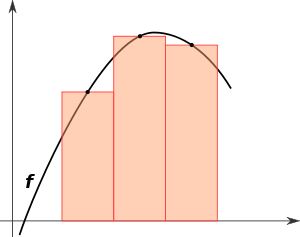
\includegraphics[width=5cm]{pic/methode_rectangles.png}
\tabularnewline 
&	\begin{tiny}Source : Wikipedia\end{tiny}\\
\end{tabular}


\end{document}